\documentclass[12pt,letterpaper]{article}
\usepackage[margin=1in]{geometry}
\usepackage{fancyhdr}
\usepackage[utf8]{inputenc}
\usepackage{palatino}
\usepackage{microtype}
\usepackage{hyperref}
\usepackage{graphicx}
\usepackage{lastpage}
\usepackage[hang,small,margin=1in]{caption}
\usepackage{titlesec}

\renewcommand{\headrulewidth}{0pt}
\fancyfoot{}
\fancyfoot[C]{\sffamily Page \thepage\ of \pageref{LastPage}}
\pagestyle{fancy}

\titleformat{\section}{\bfseries\MakeUppercase}{\arabic{\thesection}}{1em}{}
\titleformat{\subsection}{\bfseries}{\arabic{\thesection}.\arabic{\thesubsection}}{1em}{}
\titleformat{\subsubsection}{\itshape}{\arabic{\thesection}.\arabic{\thesubsection}.\arabic{\thesubsubsection}}{1em}{}

\setlength{\parindent}{0cm}
\setlength{\parskip}{1em}

\captionsetup[figure]{labelfont=it, font=it}
\captionsetup[table]{labelfont={it,sc}, font={it,sc}}

\hypersetup{colorlinks, linkcolor = black, citecolor = black, urlcolor = black}
\urlstyle{same}



\begin{document}

\fancyfoot{}
\begin{center}
    \hfill \\
    \vspace{4in}
    {\bf\Huge CS457 Project \#3 \\}
    \vspace{2in}
    {\Large Soo-Hyun Yoo \\ January 23, 2015}
\end{center}

\newpage
\fancyfoot[C]{\sffamily Page \thepage\ of \pageref{LastPage}}

\section*{Source Files}

\begin{itemize}
    \item p3.rib
    \item p3d.sl
    \item p3s.sl
\end{itemize}


\section*{Explanation}

\subsection*{p3.rib}

We declare some of the variables to be used, A, B, Height, Ramp, and
Noise\_factor, as floats. After setting some output options and light and field
of view settings, we set up our lava world. The surface and displacement
shaders are called with some values assigned to the variables declared earlier
in the file. Default color and opacity are set, and the world is transformed so
it is beautifully in view.


\subsection*{p3d.sl, p3s.sl}

The surface and displacement shader files are constructed similarly.

Both begin with definitions of some default values for the input variables.
Ellipse geometry is calculated using the given axis values.

In the surface shader, the distance from the edge of each ellipse, latitude,
and longitude values are used to calculate a HSV color value. Unlike that in
Project \#2, this object was colored with either a base color of red or
a ``land'' color of dark brown.

In the displacement shader, the same distance is instead used to displace the
surface to a certain height defined by the Ramp variable. De-defining
DISPLACEMENT\_MAPPING enables bump mapping.

In both shaders, noise is added to the scaled u and v coordinates. As all
further calculations are performed on u and v, this distorts the ellipses,
thereby the colors and displacement, according to the noise. The noise is
applied at multiple frequencies in a for loop.


\newpage
\section*{Results}

\begin{figure}[!h]
    \centering
    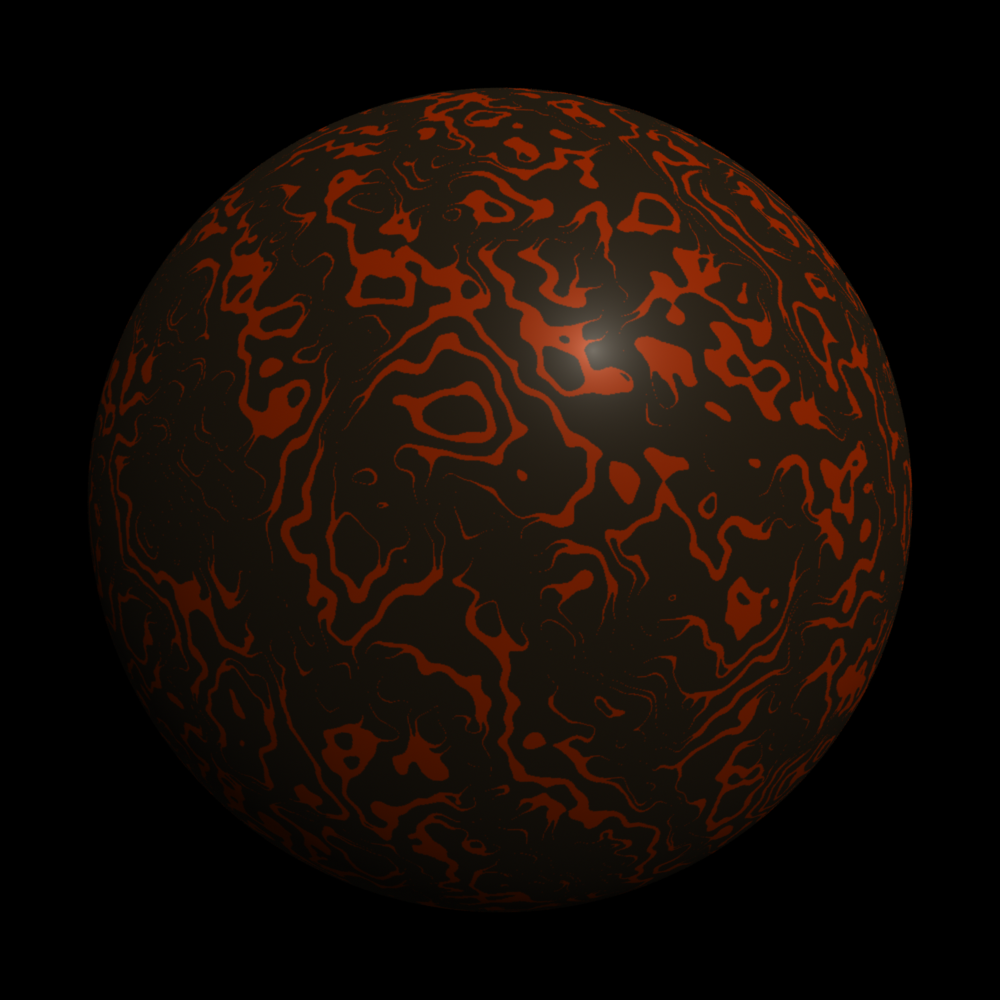
\includegraphics[width=1.0\textwidth]{img/surface_perturb.png}
    \caption{Surface perturbation at Noise\_factor = 4}
    \label{fig:ellipses}
\end{figure}

\begin{figure}[!h]
    \centering
    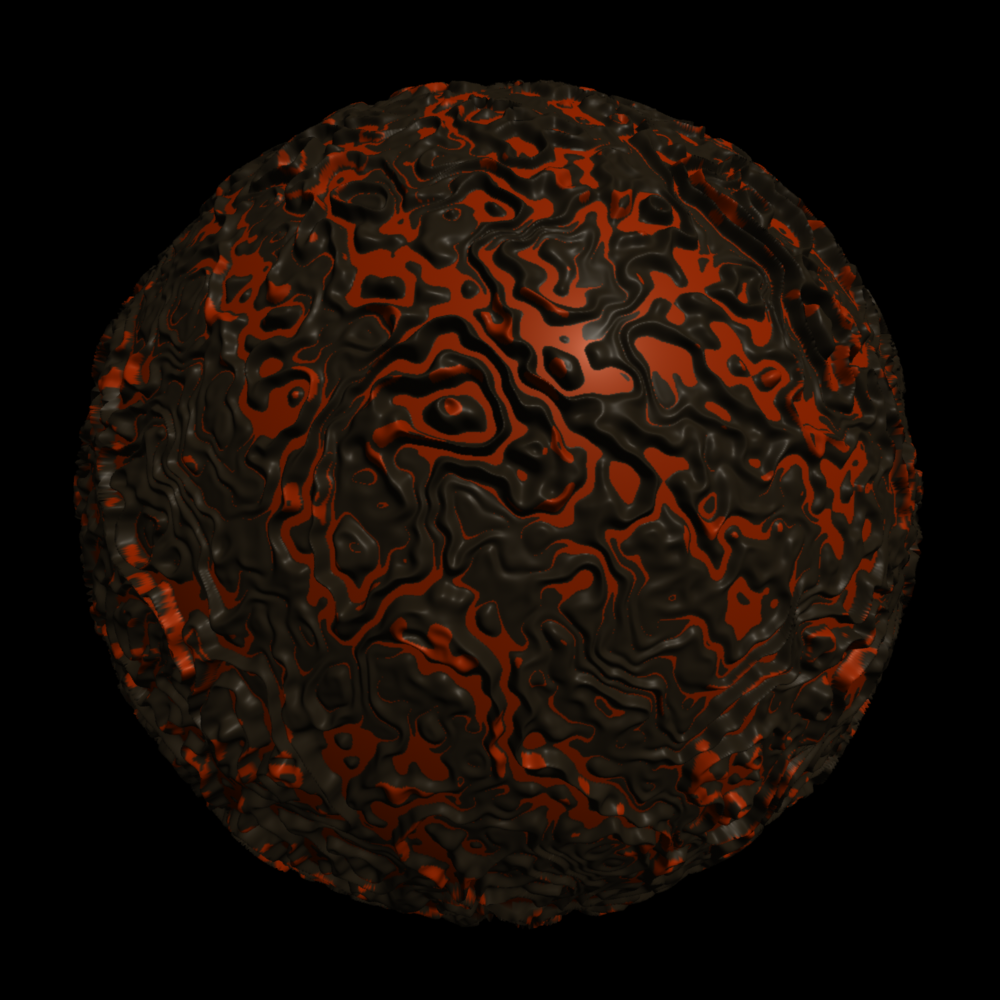
\includegraphics[width=1.0\textwidth]{img/disp_perturb.png}
    \caption{Displacement perturbation at Noise\_factor = 4. For some reason,
    the displacement interferes with the surface shader.}
\end{figure}

\begin{figure}[!h]
    \centering
    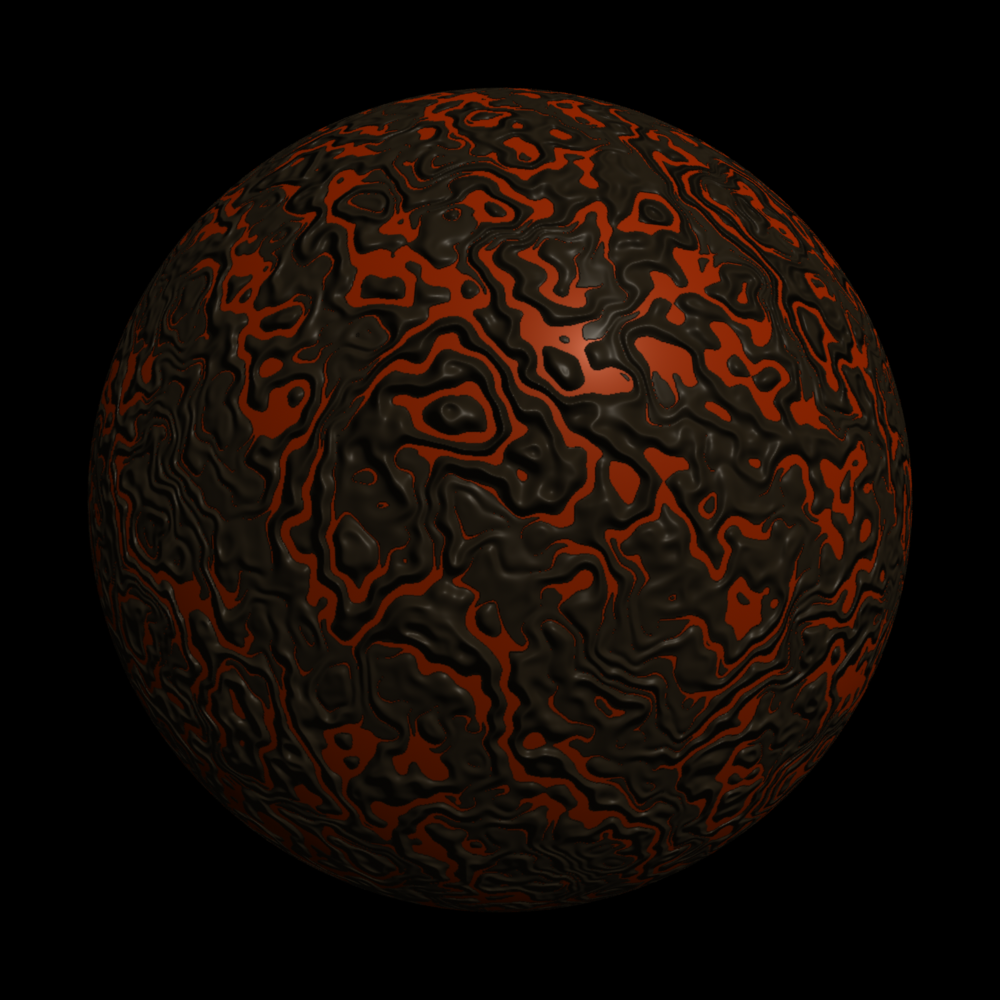
\includegraphics[width=1.0\textwidth]{img/bump.png}
    \caption{Bump mapped world}
\end{figure}

\end{document}
